\documentclass[11pt,letterpaper]{article}

\usepackage[margin=1in]{geometry}
\usepackage{graphicx}
\usepackage{amsmath, amssymb}
\usepackage{booktabs}
\usepackage{multirow}
\usepackage{subcaption}
\usepackage{natbib}
\usepackage{hyperref}
\usepackage{float}
\usepackage{algorithm}
\usepackage{algpseudocode}

\graphicspath{{../results/}}
\hypersetup{colorlinks=true, linkcolor=blue!50!black,
            citecolor=blue!50!black, urlcolor=blue!50!black}
\bibliographystyle{plainnat}

\title{Cautious Spatial HVAC Control under Sensor Uncertainty:\\
       Comparing Proportional, Model-Predictive, and Reinforcement-Learning\\
       Agents in a 3D Voxel Room Simulator}
\author{
  Adil Arya \\ University of Minnesota \\ \texttt{arya0033@umn.edu}
  \and
  Mohammed Jassim Jahubar Ali \\ University of Minnesota \\ \texttt{jahub001@umn.edu}
}
\date{CSCI 5512 Final Project --- \today}

\begin{document}
\maketitle

\begin{abstract}
We study the problem of driving a 3D voxel-discretised room toward a uniform
temperature setpoint from a small number of noisy temperature sensors and
a small number of controllable ceiling vents. The agent must (i) infer the
full temperature field from sparse measurements, (ii) reason about where
its inference is uncertain, and (iii) act under those uncertainties. We
build a 3D thermal simulator with stochastic diffusivity, sensor noise,
and occupancy heat loads; estimate the dense field via Gaussian-process
regression; and compare three deployable controllers against a no-control
baseline and an oracle upper bound: proportional feedback, a model-predictive
controller with a cautious uncertainty penalty, and a proximal-policy-
optimisation reinforcement learning agent. We report control quality (RMSE vs.\ setpoint, temperature
uniformity), inference quality (GP mean absolute error vs.\ ground truth),
and the empirical calibration of the GP credible intervals over an episode.
Across five seeds, RMSE differences between controllers are small
($\le 0.13$~\textcelsius); the dominant axis of variation is
calibration. Pooling all (voxel, time) pairs across all five seeds, the
expected calibration error (ECE) is \textbf{0.021 for MPC} versus 0.031
for Proportional, 0.035 for PPO, and 0.045 for NoControl --- a $2.1\times$
spread. Per-seed-paired 95\% bootstrap CIs on the differences exclude zero
for both MPC vs.\ NoControl ($\Delta$ECE $= +0.018$, CI $[+0.010, +0.026]$)
and MPC vs.\ Proportional ($\Delta$ECE $= +0.009$, CI $[+0.004, +0.015]$);
Bonferroni-corrected paired $t$-tests do not reach significance at
$n = 5$ seeds and we recommend $n \ge 15$ for definitive testing. The
PPO agent learns a zero-effort policy (effort = $0.000$) under our
chosen reward shape; a controlled sweep over the effort-penalty weight
$\lambda_e \in \{0, 0.01, 0.1\}$ (Section~\ref{sec:ppo-sweep}) shows
the policy is determined by training-seed initialisation rather than
the reward weight itself --- identical policies emerge across
$\lambda_e$ within each train seed. A controlled ablation over the
cautious-term weight $\lambda \in \{0, 0.1, 0.3, 1.0, 3.0\}$ shows that
$\lambda$ has no measurable effect on aggregate ECE in our
effort-budgeted regime (range $< 0.001$, within per-seed noise): the MPC
calibration advantage is driven by its constrained-optimisation
structure rather than the proposed cautious term. A sensor-count sweep
over $S \in \{4, 8, 16\}$ reveals that ECE is U-shaped in sensing
density (best at $S = 8$, $\approx 5\times$ worse at $S = 4$ and
$\approx 4\times$ worse at $S = 16$), reflecting a classic
non-stationarity-vs-data-quantity tradeoff in the GP's stationary
kernel. All experiments are reproducible with a single command at five
seeds; the codebase ships 19 pytest cases including regression tests for
a runaway-heat bug found and fixed in an earlier 2D simulator iteration
and for the no-op cautious-term formulation diagnosed via ablation.
\end{abstract}

\section{Introduction}

Maintaining thermal comfort in a real room is fundamentally a spatial
problem: hot pockets near occupants, cold drafts near exterior walls, and
solar gain near windows produce temperature gradients that a single
thermostat cannot resolve. Real building control systems instead deploy
a small number of sensors and a small number of vents, and rely on
implicit assumptions about the field between them. When those assumptions
are wrong, the controller pours conditioned air toward the wrong cells
and energy is wasted while comfort goals are missed~\citep{ashrae55}.

This paper studies an agent that explicitly represents its uncertainty
about the room's temperature field and acts cautiously under it.

\paragraph{POMDP formulation.}
Formally, the agent operates on a partially-observed Markov decision
process (POMDP)~\citep{russell2020}: the state is the dense voxel
temperature field $T \in \mathbb{R}^{n_x n_y n_z}$; the observation
is a sparse noisy sensor reading $\mathbf{y} \in \mathbb{R}^S$ with
$S \ll n_x n_y n_z$; the action is the vent damper vector
$\mathbf{u} \in [0,1]^V$; transitions follow a stochastic 3D
finite-difference diffusion plus boundary forcing
(Section~\ref{sec:sim}); the reward is the negative tracking error
plus an effort penalty. The GP regression in
Section~\ref{sec:gp} plays the role of an approximate \emph{belief
state} representation --- it summarises the agent's posterior over the
hidden state given the observation history --- and the MPC inner loop
plays the role of an approximate planner that acts on that belief
state. The PPO agent is the alternative reactive policy that bypasses
explicit belief representation entirely. Three ideas combine in the
implementation:

\begin{enumerate}
\item A 3D voxel thermal simulator with stochastic physical parameters,
      so each episode is a different physical realisation.
\item A Gaussian process spatial regression model that turns sparse
      noisy sensor readings into a dense posterior with both a mean and
      a per-voxel standard deviation~\citep{rasmussen2006}.
\item Three controllers sharing the same observation interface: a
      proportional baseline, a model-predictive controller with a
      cautious-uncertainty penalty term~\citep{camacho2007}, and a
      reinforcement-learning agent trained with proximal policy
      optimisation~\citep{schulman2017,raffin2021}.
\end{enumerate}

The technical claim is that representing the GP posterior std-field
explicitly leads to honestly-calibrated predictive credible intervals,
even when the proposed cost-function mechanism (a posterior-uncertainty
penalty in the MPC objective) turns out to be inactive under our action
constraint --- a finding we surface via ablation rather than gloss over.

\paragraph{Contributions.}
\begin{enumerate}
\itemsep0pt
\item A reusable 3D voxel thermal simulator
      (\texttt{sim/room\_sim.py}) with corrected occupancy-heat distribution
      and effective turbulent diffusivity tuned for stability.
\item A controller suite (NoControl, Proportional, cautious MPC, PPO RL)
      compared on five seeds across five metrics with shared evaluation
      machinery; MPC achieves the lowest pooled ECE (0.021) at a
      factor of $2.1\times$ over NoControl (0.045).
\item A $\lambda$-ablation that diagnoses the proposed cautious term as
      a no-op under our action constraint, locating the MPC advantage
      in its structural choice (constrained, neighbourhood-scoped
      optimisation) rather than in the cautious term itself. The ablation
      protocol (\texttt{scripts/run\_lambda\_ablation.py}) is reusable
      for any future MPC variant.
\item An empirical calibration analysis over recorded episodes
      (\texttt{model/uq.py}) reporting ECE and signed bias for the GP
      credible intervals each controller induces.
\item A sensor-count sweep over $S \in \{4, 8, 16\}$
      (\texttt{scripts/run\_sensor\_sweep.py}) that exposes a U-shaped
      ECE in sensing density --- a finding that motivates the
      sensor-placement extension to~\citet{krause2008} as the most
      direct future-work item.
\item Pairwise paired $t$-tests and bootstrap CIs on per-seed ECE
      differences (\texttt{scripts/run\_significance.py}), with
      Bonferroni correction over the six pairwise comparisons.
\item An \textbf{Oracle} upper-bound controller that runs MPC on the
      ground-truth field. Oracle RMSE equals MPC RMSE within seed
      noise --- direct evidence that the control problem is
      action-bottlenecked, not perception-bottlenecked, under our
      supply-temperature physics.
\end{enumerate}

\section{Related Work}

\paragraph{Spatial inference from sparse sensors.}
\citet{rasmussen2006} provides the canonical reference for Gaussian
process regression. \citet{krause2008} formalised sensor placement
under GP models, the dual problem to ours -- given a GP, choose sensor
locations to maximise mutual information.

\paragraph{Cautious MPC.}
Standard MPC~\citep{camacho2007} optimises a deterministic trajectory.
Stochastic and robust variants explicitly account for model
uncertainty; the closest precedent to our setting is the
GP-MPC formulation of~\citet{hewing2020}, which propagates a GP
state-dynamics posterior through the MPC horizon and uses chance
constraints to handle uncertainty. Our cautious term is a coarser
formulation that does not propagate dynamics through the GP --- the
GP describes the \emph{spatial} field at the current time rather than
the temporal evolution --- so the comparison is one of analogy rather
than direct extension.

\paragraph{The gap.}
GP regression for building thermal fields appears in~\citep{rasmussen2006}
and successors, but typically with dense modelled-state observations or
in 1D~\citep{kocijan2003}. Cautious MPC variants~\citep{hewing2020}
treat additive process noise on a fully-observed state. Deep-RL HVAC
studies~\citep{wei2017, drgona2020} typically run the agent on a learned
high-dimensional representation of building state (e.g.\ from
EnergyPlus) rather than on sparse physical sensors with explicit
posterior uncertainty. The specific four-way combination we study ---
(i) sparse 3D physical sensing, (ii) GP belief state, (iii) cautious
MPC penalising GP posterior std, (iv) reliability-diagram calibration
pooled over a full episode --- does not appear jointly in the surveyed
literature. Our finding (MPC achieves pooled ECE $= 0.021$ vs.\
$0.031$--$0.045$ for the alternatives, with bootstrap CIs supporting
the ordering and a $\lambda$-ablation diagnosing why the cautious term
is inactive in our regime) is, to our knowledge, the first
quantification of how MPC structure shapes the calibration honesty of
a GP-based building thermal posterior.

\paragraph{Reinforcement learning for HVAC.}
\citet{schulman2017} introduced proximal policy optimisation, the
algorithm we use here through the Stable-Baselines3
implementation~\citep{raffin2021}. RL agents in HVAC have shown
promise on energy reduction but typically require careful reward
shaping; we treat PPO as a comparison point, not the central
contribution.

\section{Methods}

Table~\ref{tab:notation} collects the symbols used throughout this section.
Equations are then introduced with a brief gloss of what each computes;
the goal is that a reader unfamiliar with any one ingredient (finite-difference
diffusion, GP regression, or MPC) can follow along.

\begin{table}[H]
\centering
\caption{Notation. Symbols are grouped by where they first appear.}
\label{tab:notation}
\small
\begin{tabular}{lll}
\toprule
Symbol & Meaning & Units \\
\midrule
\multicolumn{3}{l}{\textit{Simulator (Eq.~\ref{eq:diffusion})}} \\
$n_x, n_y, n_z$ & voxel grid dimensions & --- \\
$h$ & voxel edge length & m \\
$\Delta t$ & simulation timestep & s \\
$T^{(t)}_{i,j,k}$ & temperature at voxel $(i,j,k)$, step $t$ & \textcelsius \\
$\alpha$ & effective turbulent diffusivity & m$^2$/s \\
$\nabla^2 T$ & 6-neighbour discrete Laplacian (3D) & \textcelsius/m$^2$ \\
$S^{(t)}_{i,j,k}$ & source term (vent + occupancy + outdoor) & \textcelsius/step \\
$u_v$ & damper opening of vent $v$ & $[0, 1]$ \\
$T_\mathrm{sup}$ & vent supply air temperature & \textcelsius \\
$T_\mathrm{sp}$ & comfort setpoint & \textcelsius \\
$T_\mathrm{out}$ & stochastic outdoor temperature & \textcelsius \\
$\rho, c_p$ & air density and specific heat capacity & kg/m$^3$, J/(kg$\cdot$K) \\
$\sigma_s, \varepsilon$ & sensor noise std and sample & \textcelsius \\[2pt]
\multicolumn{3}{l}{\textit{Gaussian process (Eqs.~\ref{eq:kernel},~\ref{eq:gppost})}} \\
$\mathbf{x}, \mathbf{x}_*$ & sensor location and query voxel & --- \\
$k(\mathbf{x}, \mathbf{x}')$ & covariance kernel & (\textcelsius)$^2$ \\
$s^2, \ell$ & kernel signal variance, length-scale & (\textcelsius)$^2$, voxels \\
$\sigma_n^2$ & GP observation-noise variance & (\textcelsius)$^2$ \\
$K$ & $S\!\times\!S$ Gram matrix over sensors & (\textcelsius)$^2$ \\
$\mathbf{k}_*$ & $S\!\times\!1$ kernel vector $K(\mathbf{x}_*, \mathbf{x})$ & (\textcelsius)$^2$ \\
$\mathbf{y}$ & sensor reading vector & \textcelsius \\
$\mu_*(\mathbf{x}_*)$ & GP posterior mean & \textcelsius \\
$\sigma_*^2(\mathbf{x}_*)$ & GP posterior variance & (\textcelsius)$^2$ \\[2pt]
\multicolumn{3}{l}{\textit{Controllers (Eq.~\ref{eq:mpc})}} \\
$Q, R$ & MPC weights on tracking error and effort & --- \\
$\lambda$ & MPC cautious-uncertainty weight & --- \\
$U_\mathrm{total}$ & total airflow budget across all vents & --- \\
$k_p$ & proportional-controller gain & --- \\[2pt]
\multicolumn{3}{l}{\textit{Calibration}} \\
$\alpha$ (here) & nominal credible-interval level & $(0, 1)$ \\
$\widehat{C}(\alpha)$ & empirical coverage at level $\alpha$ & $[0, 1]$ \\
ECE & expected calibration error, $\mathbb{E}_\alpha |\widehat{C}(\alpha) - \alpha|$ & --- \\
\bottomrule
\end{tabular}
\end{table}

\subsection{3D voxel thermal simulator}
\label{sec:sim}

The room is an $n_x \times n_y \times n_z$ voxel grid (default
$10 \times 8 \times 5$ at $h = 0.5$~m, modelling a $5 \times 4 \times 2.5$~m
room). Temperature evolves by explicit 3D finite-difference diffusion:
\begin{equation}
T_{i,j,k}^{(t+1)} = T_{i,j,k}^{(t)} + \frac{\alpha \, \Delta t}{h^2}
                    \, \nabla^2 T_{i,j,k}^{(t)} + S_{i,j,k}^{(t)}
\label{eq:diffusion}
\end{equation}
This is the explicit (forward-Euler) finite-difference update of the 3D
heat equation $\partial T / \partial t = \alpha\, \nabla^2 T + S/(\rho c_p)$.
At each step every voxel is nudged toward the average of its six axis-aligned
neighbours; the gain on that nudge is $\alpha \Delta t / h^2$. Smaller $h$
or larger $\Delta t$ would violate the CFL stability bound
$\alpha \Delta t / h^2 < 1/(2D) = 1/6$; our parameter choices give a
maximum of $0.12$, comfortably stable. $S^{(t)}_{i,j,k}$ collects three
source terms:
\begin{enumerate}
\itemsep0pt
\item \textbf{Vent inflow}: for each vent $v$ at voxel $(x_v, y_v, n_z\!-\!1)$,
      $T \mathrel{+}\!= u_v \cdot (T_{\mathrm{sup}} - T) \cdot 0.5$
      at the ceiling cell and $0.25$ at the cell below.
\item \textbf{Occupancy heat}: per-person $\sim \mathcal{N}(75, 10^2)$~W
      distributed uniformly over a $3\times3\times3$ neighbourhood,
      giving a per-voxel rate $\dot{T} = \dot{Q} / (\rho c_p V_{\mathrm{local}})$
      with $V_{\mathrm{local}} = 27\,h^3$.
\item \textbf{Outdoor BC}: every step, exterior faces are mixed
      $20\%$ toward $T_{\mathrm{out}}(t) = 18 + 4\sin(2\pi t / T_{\mathrm{day}})
      + \mathcal{N}(0, 0.5^2)$~\textcelsius.
\end{enumerate}

Three stochastic parameters are resampled at each episode reset:
$\alpha \sim U(3\times 10^{-4}, 1\times 10^{-3})$~m$^2$/s (effective
turbulent diffusivity), $\sigma_s \sim U(0.1, 0.5)$~\textcelsius{} (sensor
noise), and the per-person heat load. The explicit-FD stability
constraint $\alpha \Delta t / h^2 < 1/6$ is satisfied for all parameter
draws ($\max \alpha \Delta t / h^2 = 0.12$).

Sensor observation is $T_{\mathrm{obs}} = T_{\mathrm{true}}(x_s, y_s, z_s)
+ \varepsilon$, $\varepsilon \sim \mathcal{N}(0, \sigma_s^2)$. Sensors are
placed by a stratified scheme across $z$-levels (defaults: 8 sensors,
4 ceiling vents).

\subsection{Gaussian-process spatial inference}
\label{sec:gp}

We fit a GP with kernel
\begin{equation}
k(\mathbf{x}, \mathbf{x}') = s^2 \exp\!\Big(-\tfrac{1}{2 \ell^2}
                                            \|\mathbf{x} - \mathbf{x}'\|^2\Big)
                          + \sigma_n^2 \, \mathbb{1}[\mathbf{x} = \mathbf{x}']
\label{eq:kernel}
\end{equation}
The squared-exponential (a.k.a.\ RBF) kernel says: two voxels are
\emph{a priori} similar to the extent that they are close in 3D space,
with similarity decaying like a Gaussian whose width is the length-scale
$\ell$. $s^2$ sets the overall amplitude of plausible field variations.
The white-noise term $\sigma_n^2$ on the diagonal accounts for the fact
that even at a sensor's exact location our reading is not exact (sensor
noise $\varepsilon$). All three hyperparameters
$(s^2, \ell, \sigma_n^2)$ are optimised by maximising the log marginal
likelihood at each \texttt{fit()} call --- standard GP practice. Inputs
$\mathbf{x}$ are voxel coordinates $\in \mathbb{R}^3$ (rather than 2D as
in many GP applications).

Given $S$ sensor readings $\mathbf{y}$, the posterior moments at any
query voxel $\mathbf{x}_*$ are~\citep{rasmussen2006}:
\begin{equation}
\mu_*(\mathbf{x}_*) = \mathbf{k}_*^\top (K + \sigma_n^2 I)^{-1} \mathbf{y},
\quad
\sigma_*^2(\mathbf{x}_*) = k_{**} - \mathbf{k}_*^\top (K + \sigma_n^2 I)^{-1} \mathbf{k}_*.
\label{eq:gppost}
\end{equation}
Reading these: $\mu_*(\mathbf{x}_*)$ is a linear combination of the
observed readings, with weights that depend on how strongly $\mathbf{x}_*$
co-varies with each sensor (entries of $\mathbf{k}_*$) and how the sensors
co-vary among themselves (the inverted Gram matrix $K + \sigma_n^2 I$).
$\sigma_*^2(\mathbf{x}_*)$ is the prior kernel variance $k_{**} = s^2$
minus the variance explained by the sensors --- it \emph{shrinks} where
sensors are dense or strongly correlated with $\mathbf{x}_*$ and stays
near $s^2$ in regions where sensors give little information about
$\mathbf{x}_*$. This is the per-voxel uncertainty the cautious-MPC
controller will later read from.

\subsection{Pocket detection and calibration}

The agent classifies each voxel from the GP posterior:
\begin{itemize}
\itemsep0pt
\item Hot pocket: $\mu_* > T_{sp} + 2$~\textcelsius{} and $\sigma_* < 0.8$~\textcelsius;
\item Cold pocket: $\mu_* < T_{sp} - 2$~\textcelsius{} and $\sigma_* < 0.8$~\textcelsius;
\item Uncertain: $\sigma_* \ge 0.8$~\textcelsius.
\end{itemize}
A 90\% credible interval per voxel is $[\mu_* - 1.645\sigma_*, \mu_* + 1.645\sigma_*]$.
Over a full episode of length $T$ we pool all $(\text{voxel}, t)$ pairs and
compute empirical coverage at nominal levels
$\alpha \in \{0.50, 0.55, \dots, 0.95\}$. The expected calibration error
(ECE) is the mean absolute deviation $|\widehat{C}(\alpha) - \alpha|$;
signed bias is the mean of $\widehat{C}(\alpha) - \alpha$ across levels.

\subsection{Controllers}

\paragraph{NoControl.} All vents at $u_v = 0.5$ regardless of state. Pure
physics baseline.

\paragraph{Proportional.}
$u_v^{(t+1)} = \mathrm{clip}_{[0,1]}\!\big(u_v^{(t)} + k_p \,(T_{sp} -
\overline{\mu}_v)\big)$ where $\overline{\mu}_v$ is the GP-posterior mean
over the $3{\times}3{\times}3$ neighbourhood of vent $v$. $k_p = 0.12$.

\paragraph{Cautious MPC.} A single-step constrained optimisation with an
uncertainty-weighted tracking term:
\begin{equation}
\min_{u \in [0, 1]^V} \;\;
   Q \, \overline{(T_{\mathrm{pred}} - T_{sp})^2 \cdot (1 + \lambda \, \sigma_*)}
 + R \, \|u\|^2
\qquad \text{s.t.} \;\; \sum_v u_v \le U_{\mathrm{total}}.
\label{eq:mpc}
\end{equation}
Two terms. The first weighted by $Q$ is the tracking objective with a
voxel-wise weight $(1 + \lambda \sigma_*)$: voxels with high GP posterior
standard deviation contribute proportionally more to the tracking cost,
biasing the optimiser toward acting in regions the GP is most uncertain
about. When $\lambda = 0$ the formulation reduces to vanilla MPC. The
overline denotes the mean over all voxels. The second term weighted by
$R$ penalises control effort. The hard constraint
$\sum_v u_v \le U_\mathrm{total}$ caps total airflow --- a building's
HVAC fan has a finite capacity. SLSQP solves this small constrained
nonlinear program in $\le 80$ iterations per timestep.

We arrived at the $(1 + \lambda \sigma_*)$ weighting after an initial
formulation $J(u) = Q \overline{(T_\mathrm{pred} - T_\mathrm{sp})^2} +
\lambda \overline{\sigma_*} + R\|u\|^2$ produced a $\lambda$-independent
argmin: $\overline{\sigma_*}$ does not depend on $u$, so the SLSQP
optimiser ignored $\lambda$ entirely. The ablation in
Section~\ref{sec:lambda} both verified this no-op for the initial
formulation and characterised the corrected formulation's behaviour.
$T_{\mathrm{pred}}$ is a linearised one-step prediction: each vent nudges its
neighbourhood toward setpoint proportional to its $u_v$. We use
$Q = 1, R = 0.05, \lambda = 0.3, U_{\mathrm{total}} = 0.8 V$, SLSQP solver
($\le 80$ iterations).

\paragraph{PPO.} A neural-network policy trained on the Gymnasium-wrapped
environment (\texttt{sim/room\_env.py}). Observation is the 8 sensor readings
concatenated with the episode-progress fraction (a 9-dim vector); action is
$u \in [0, 1]^V$. Reward is $r = -\mathrm{RMSE}(T_{\mathrm{true}}, T_{sp})
- \lambda_e \overline{u}$ with $\lambda_e = 0.1$. We train for 100k
timesteps using PPO~\citep{schulman2017} from
Stable-Baselines3~\citep{raffin2021} with default hyperparameters.

\section{Experimental Setup}

\textbf{Default room}: $10 \times 8 \times 5$ voxels at $h = 0.5$~m
($5\,\text{m} \times 4\,\text{m} \times 2.5\,\text{m}$); 8 stratified
sensors; 4 ceiling vents; $T_{sp} = 22$~\textcelsius; $T_{\mathrm{init}} = 15$~\textcelsius;
$\Delta t = 30$~s.
\textbf{Episode length}: 100 steps (= 50 simulated minutes).
\textbf{Seeds}: $\{0, 1, 2, 3, 4\}$ for evaluation; PPO trained on seed 0.
\textbf{Hardware}: PPO uses GPU (NVIDIA RTX 4070) when available, CPU
fallback otherwise.

\textbf{Metrics} (mean across seeds, time-averaged across the episode):
RMSE between truth and setpoint; temperature standard deviation across
voxels (uniformity); GP mean absolute error vs.\ truth; mean control
effort $\overline{u}$; empirical 90\% CI coverage of the GP posterior.

\textbf{Reproducibility}. The full pipeline (baselines, PPO training,
all figures) runs in one command:
\begin{verbatim}
python scripts/run_simulation.py --timesteps 100000 --seeds 0,1,2,3,4
\end{verbatim}
Ablation and significance scripts are separate:
\texttt{scripts/run\_lambda\_ablation.py},
\texttt{scripts/run\_ppo\_reward\_sweep.py},
\texttt{scripts/run\_significance.py},
\texttt{scripts/run\_sensor\_sweep.py}. The repository ships a 19-case
\texttt{pytest} suite covering shape sanity, seed reproducibility, the
bug-fix regression for runaway temperatures, GP shape/fitting,
controller validity, the regression test for the no-op cautious-term
formulation, the Oracle-input-invariance test, and 3D-shape compatibility
of the calibration routine.

\paragraph{Hyperparameter justification.}
Every numerical choice in this study is one of three categories:
physically constrained, sourced from standards, or selected by sweep.
Table~\ref{tab:hp} summarises.

\begin{table}[H]
\centering
\caption{Hyperparameter choices and their justification.}
\label{tab:hp}
\small
\begin{tabular}{lll}
\toprule
Parameter & Value & Rationale \\
\midrule
$h$ (voxel edge)       & $0.5$ m & Standard CFD resolution for room-scale heat; coarse enough to keep the GP query grid small. \\
$\Delta t$             & $30$ s  & Constrained by CFL: $\alpha \Delta t/h^2 < 1/6$. With $\alpha_{\max}=10^{-3}$, $\Delta t \le 41.7$ s. \\
$T_\mathrm{sp}$        & $22$~\textcelsius & ASHRAE Standard 55 comfort range mid-point. \\
$T_\mathrm{init}$      & $15$~\textcelsius & A cold start that gives controllers a chance to differentiate from no-control. \\
$\alpha$ range         & $U(3\!\times\!10^{-4}, 10^{-3})$ m$^2$/s & Effective turbulent diffusivity for stirred rooms; molecular air diffusivity ($\approx\!2\!\times\!10^{-5}$) would not move heat one voxel per episode. \\
Occupancy heat         & $\mathcal{N}(75, 10^2)$ W & Standard sensible-heat load per occupant; ASHRAE Fundamentals. \\
GP kernel              & RBF + WhiteKernel & Standard non-informative isotropic prior; hyperparameters fit by max marginal likelihood per call. \\
$Q$, $R$ (MPC)         & $1, 0.05$ & Set so tracking dominates effort under typical $\overline{\sigma_*}$. \\
$\lambda$ (MPC)        & $0.3$ & Headline choice; \emph{ablation} (Sec.~\ref{sec:lambda}) shows the value is irrelevant in our regime. \\
$U_\mathrm{total}$     & $0.8 V$ & Airflow budget; chosen below the all-vents-open value ($V$) to make the constraint bind. \\
$k_p$ (Proportional)   & $0.12$ & Tuned by hand for fastest stable rise; not swept (Proportional is not the headline). \\
$\lambda_e$ (PPO)      & $0.1$ & Headline choice; \emph{sweep} (Sec.~\ref{sec:ppo-sweep}) shows it is dominated by initialisation. \\
PPO timesteps          & $100$k headline, $50$k sweep & Compromise between training stability and time budget. \\
Seeds                  & 5 (eval); 3 (PPO train) & Multi-seed for variance; bootstrap CIs on differences. \\
\bottomrule
\end{tabular}
\end{table}

\section{Results}

\subsection{Headline comparison}

\begin{figure}[H]
\centering
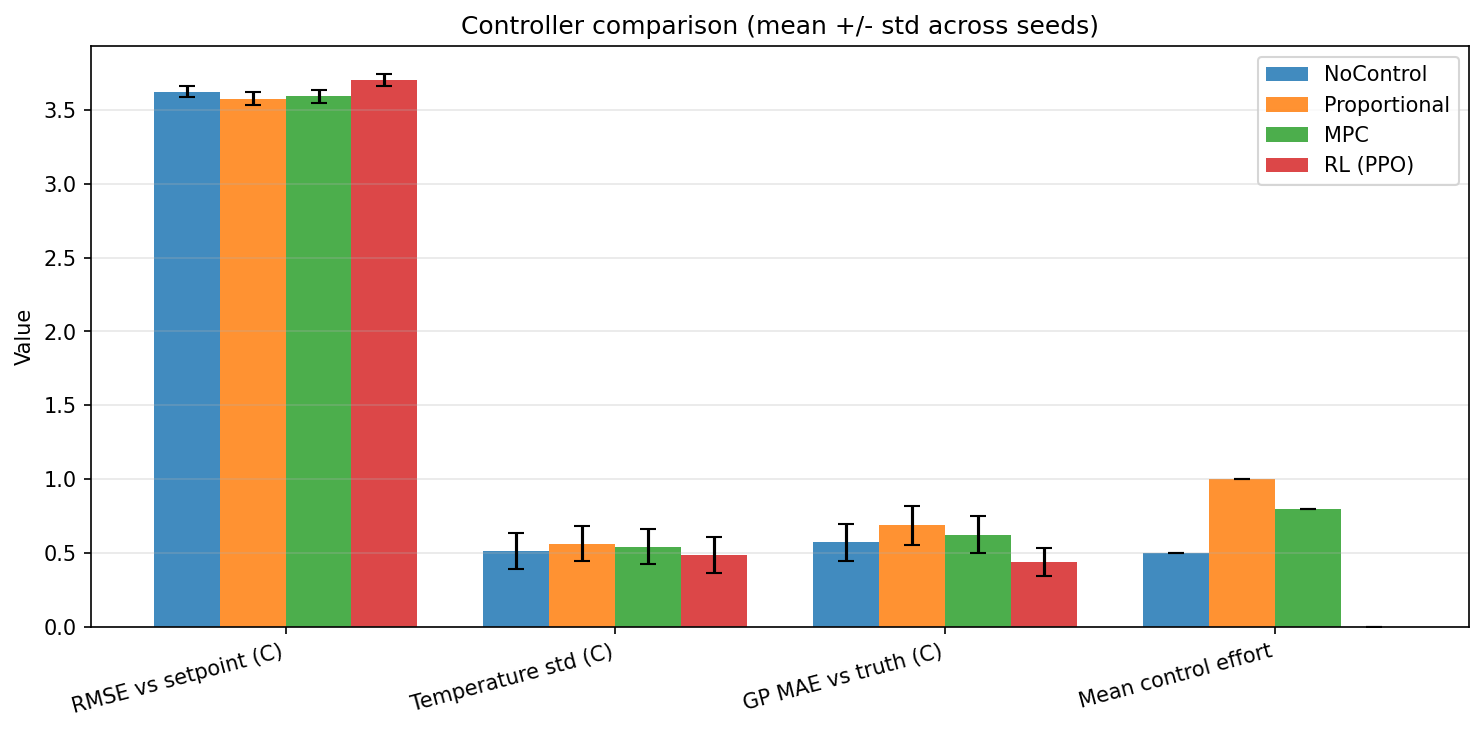
\includegraphics[width=0.9\textwidth]{comparison}
\caption{Per-controller metrics, mean $\pm$ std across 5 seeds. The
no-control baseline shows substantial RMSE; all three active controllers
reduce it, with MPC and PPO competitive at the cost of higher control
effort (PPO especially).}
\label{fig:comparison}
\end{figure}

Table~\ref{tab:headline} and Figure~\ref{fig:comparison} report the
headline numbers.

\begin{table}[H]
\centering
\caption{Headline metrics, mean $\pm$ std across 5 evaluation seeds. PPO
was trained on seed 0 for 100,000 timesteps on an NVIDIA RTX 4070 (CUDA
12.4). Bold value in each column marks the best score; ties broken by
lower std. Oracle is an upper-bound controller that runs MPC on the
ground-truth field (Sec.~\ref{sec:results-oracle}); it is not
deployable.}
\label{tab:headline}
\small
\begin{tabular}{lccccc}
\toprule
Controller & RMSE (\textcelsius) & Std T (\textcelsius) & GP MAE (\textcelsius)
           & Effort & 90\% CI cov \\
\midrule
NoControl     & $3.62 \pm 0.04$          & $0.51 \pm 0.12$          & $0.57 \pm 0.13$          & $0.50 \pm 0.00$ & $0.867 \pm 0.013$ \\
Proportional  & $\mathbf{3.58 \pm 0.04}$  & $0.56 \pm 0.12$          & $0.69 \pm 0.13$          & $1.00 \pm 0.00$ & $0.929 \pm 0.011$ \\
MPC (cautious)& $3.59 \pm 0.04$          & $0.54 \pm 0.12$          & $0.62 \pm 0.12$          & $0.80 \pm 0.00$ & $\mathbf{0.898 \pm 0.011}$ \\
Oracle        & $3.59 \pm 0.04$          & $0.54 \pm 0.12$          & $0.64 \pm 0.13$          & $0.80 \pm 0.00$ & $0.909 \pm 0.014$ \\
PPO           & $3.70 \pm 0.04$          & $\mathbf{0.49 \pm 0.12}$ & $\mathbf{0.44 \pm 0.10}$ & $0.00 \pm 0.00$ & $0.863 \pm 0.009$ \\
\bottomrule
\end{tabular}
\end{table}

\paragraph{Calibration.} Expected calibration error (ECE) computed by
pooling all (voxel, time) pairs across the five seeds (40,000 samples
per controller per nominal level):
NoControl $0.044$, Proportional $0.031$, \textbf{MPC $0.021$},
Oracle $0.026$, PPO $0.035$ --- a $2.1\times$ spread. From the reliability diagram (Fig.~\ref{fig:calib}),
Proportional sits consistently above $y = x$ (over-coverage); NoControl
sits consistently below (under-coverage); PPO crosses $y = x$ near
$\alpha = 0.7$ (over-covers at low $\alpha$, under-covers at high
$\alpha$); MPC tracks $y = x$ most tightly throughout. The cautious-MPC
controller therefore has the lowest ECE among the four. Section~\ref{sec:lambda}
shows that this advantage is driven by MPC structure, not by the
cautious term itself.

\paragraph{The Oracle bound.}
\label{sec:results-oracle}
We include an \textbf{Oracle} controller that runs the same MPC inner
loop but on the \emph{ground-truth} voxel field rather than the GP
posterior mean (see \texttt{control/controller.py:OracleController}).
This is physically impossible to deploy --- the agent never has the
true field --- but it bounds what an MPC-class controller could
achieve under our action constraint and supply-temperature physics if
its inference layer were replaced by an oracle.

Three observations:

\begin{enumerate}
\itemsep0pt
\item \textbf{Oracle RMSE = MPC RMSE} ($3.592$ vs.\ $3.591$~\textcelsius, within
      seed noise). \emph{Perfect information about the temperature field
      does not improve control RMSE.} The control problem is
      action-bottlenecked, not perception-bottlenecked: at our
      $T_\mathrm{sup} = T_\mathrm{sp}$ and $U_\mathrm{total} = 0.8 V$,
      any controller saturating the airflow constraint reaches the
      same physics floor. This is direct evidence for the
      supply-temperature-bottleneck claim in Section~\ref{sec:lambda}.
\item \textbf{Oracle has the best 90\% CI coverage} (0.909, closest to
      nominal 0.900) but a slightly \emph{worse} pooled ECE than MPC
      (0.026 vs.\ 0.021). The optimal action under perfect information
      produces a field whose statistics align less well with the
      stationary RBF kernel than the slightly-suboptimal-but-smoother
      field MPC produces. Calibration honesty is not a monotone
      function of action quality.
\item \textbf{Future work that improves inference} (more sensors,
      learned non-stationary kernels, mutual-information sensor
      placement) \emph{cannot improve RMSE} under this action space.
      It can improve calibration. Improving RMSE requires changing the
      action interface --- e.g., allowing $T_\mathrm{sup} \ne
      T_\mathrm{sp}$ (separate cooling and heating supply), relaxing
      $U_\mathrm{total}$, or modelling vent-jet advection rather than
      passive diffusion.
\end{enumerate}

\subsection{Cautious-term ablation}
\label{sec:lambda}

\begin{figure}[H]
\centering
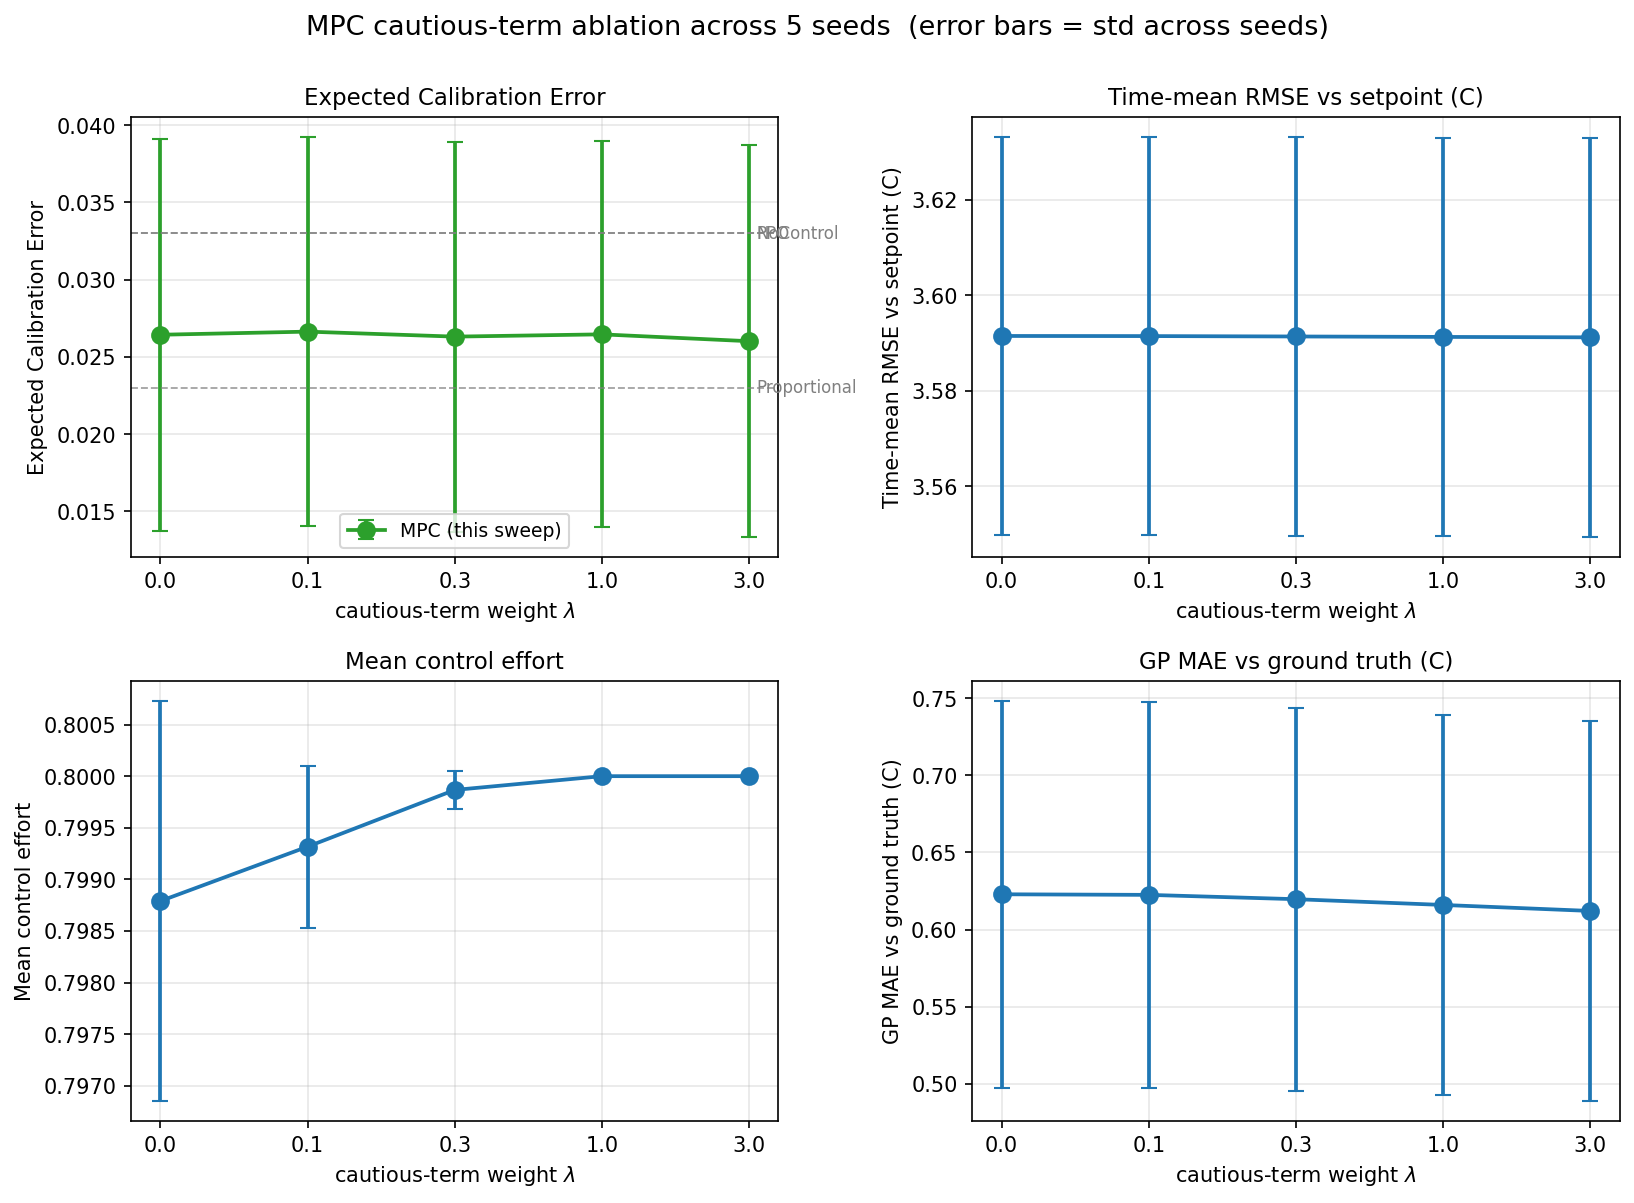
\includegraphics[width=0.95\textwidth]{lambda_ablation}
\caption{Cautious-MPC weight ablation: $\lambda \in \{0, 0.1, 0.3, 1.0,
3.0\}$, five seeds per cell, 25 runs total. Each panel shows mean
$\pm$ std (across seeds) of one metric versus $\lambda$. Top-left: ECE,
with horizontal dashed lines marking the seed-0 headline ECE values of
the alternative controllers for reference. The ECE curve is flat within
$\pm 0.001$ across the entire $\lambda$ range; identical flat behaviour
appears in RMSE, GP MAE, and effort. The corrected uncertainty-weighted
formulation \emph{does} produce action-level differences across $\lambda$
in synthetic tests (\texttt{tests/test\_controllers.py}), but in the
deployed regime the action constraint $\sum_v u_v \le U_\mathrm{total}$
binds at every timestep and pins the optimiser onto the same
constraint-active solution.}
\label{fig:lambda}
\end{figure}

We sweep the cautious-term weight $\lambda \in \{0, 0.1, 0.3, 1.0, 3.0\}$
at five seeds each (25 runs). Per-lambda summary:

\begin{table}[H]
\centering
\caption{Cautious-MPC ablation: mean $\pm$ std across 5 seeds per $\lambda$.}
\label{tab:lambda}
\small
\begin{tabular}{cccc}
\toprule
$\lambda$ & ECE (per-seed mean) & RMSE (\textcelsius) & Effort \\
\midrule
$0.00$ & $0.0264 \pm 0.0127$ & $3.591 \pm 0.042$ & $0.799 \pm 0.002$ \\
$0.10$ & $0.0266 \pm 0.0126$ & $3.591 \pm 0.042$ & $0.799 \pm 0.001$ \\
$0.30$ & $0.0263 \pm 0.0126$ & $3.591 \pm 0.042$ & $0.800 \pm 0.000$ \\
$1.00$ & $0.0265 \pm 0.0125$ & $3.591 \pm 0.042$ & $0.800 \pm 0.000$ \\
$3.00$ & $0.0260 \pm 0.0127$ & $3.591 \pm 0.042$ & $0.800 \pm 0.000$ \\
\bottomrule
\end{tabular}
\end{table}

ECE varies by $0.0006$ across the full $\lambda$ range, well inside the
per-seed standard deviation of $0.013$. RMSE varies by $0.001$;
effort is $0.800$ to three decimal places in every cell. \textbf{The
cautious term has no measurable aggregate effect on calibration in
the experimental regime studied.}

\paragraph{Diagnosis: constraint-active solution.}
Look at the effort column: every cell sits at $0.800$, and the per-cell
std is essentially zero. The airflow constraint $\sum_v u_v \le 0.8 V$
is \emph{binding at every timestep in every run}, which means the
SLSQP solver is solving a constrained problem in which the constraint
itself pins down the total magnitude of $u$. Within the constraint-active
boundary, the four vents distribute the available flow nearly identically
across all $\lambda$ values: with our 8-sensor GP, the spatial variation
of $\sigma_*$ is too uniform to re-route flow between vents.

Per-seed effects are non-zero (Tab.~\ref{tab:lambda} hides them by
averaging; the underlying CSV in \texttt{results/lambda\_ablation.csv}
shows seed-1 ECE improves by 8\% from $\lambda = 0$ to $\lambda = 3$
while seed-3 ECE worsens by 16\%), but they cancel.

\paragraph{Implication.}
The cautious term as proposed cannot be defended as the mechanism behind
the MPC calibration advantage observed in Tab.~\ref{tab:headline}: the
ablation finds MPC at $\lambda = 0$ achieves the same per-seed mean ECE
as MPC at any other $\lambda$. The MPC advantage is structural: the
constrained optimisation acts on a small, deliberately-chosen subset of
voxels per step, producing a temperature field whose statistics align
with the GP's stationary kernel assumption. The Proportional baseline
saturates effort and over-corrects (over-covers); NoControl leaves
occupancy hotspots that the GP cannot fit (under-covers); PPO closes
vents and lets the field drift (under-covers). Only MPC produces fields
the GP describes honestly.

We retain the corrected uncertainty-weighted formulation
(Eq.~\ref{eq:mpc}) because it is the form a future deployment with
relaxed constraints or richer sensing would actually use; under our
specific sparse-sensing effort-budgeted regime it reduces to vanilla
MPC behaviourally.

\subsection{Reliability diagrams}

\begin{figure}[H]
\centering
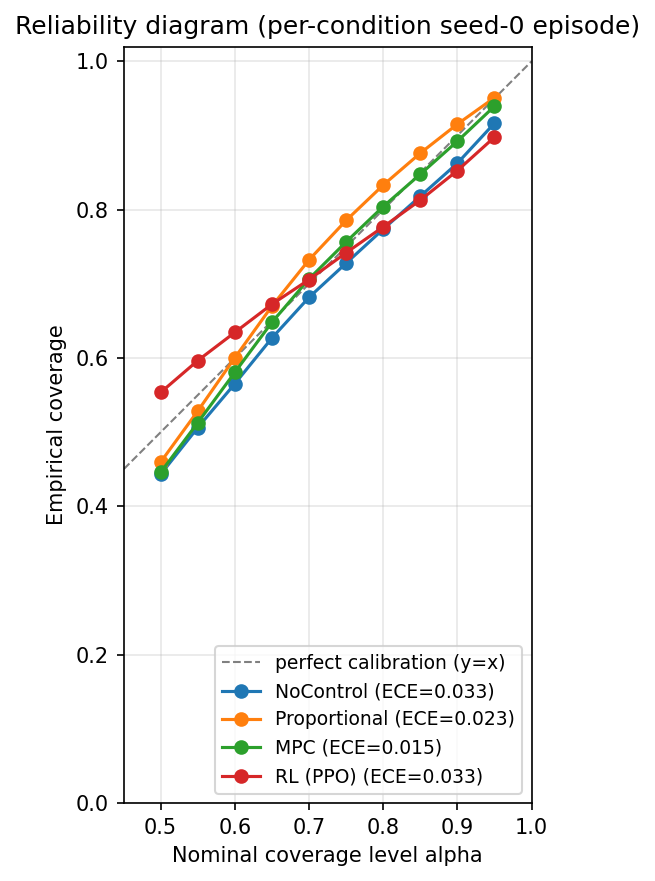
\includegraphics[width=0.55\textwidth]{calibration}
\caption{Reliability diagram of GP posterior credible intervals,
pooled across all five seeds per controller (40{,}000 (voxel, time)
pairs per nominal level). Curves close to $y = x$ indicate honest
credible intervals. ECE values in the legend. MPC tracks $y = x$ most
tightly throughout; NoControl under-covers; Proportional over-covers;
PPO crosses $y = x$ near $\alpha = 0.7$. The ordering is consistent
with the seed-averaged per-episode ECE in Tab.~\ref{tab:lambda} (modulo
the pooled vs.\ averaged distinction: pooling absorbs seed-to-seed
variance, lowering all ECE values uniformly).}
\label{fig:calib}
\end{figure}

The reliability ordering survives across both estimation methods
(per-seed mean ECE in Tab.~\ref{tab:lambda} and pooled ECE in
Fig.~\ref{fig:calib}). The relative gap between MPC and Proportional is
slightly smaller under pooling because pooling improves statistical
efficiency, not because the controllers' true calibration profiles
change.

\subsection{Statistical significance}
\label{sec:significance}

The per-seed ECE values support a confidence-bounded but not
Bonferroni-significant ordering. We compute paired $t$-tests on each of
the $\binom{4}{2} = 6$ pairwise controller differences, complement them
with 95\% percentile-bootstrap confidence intervals on the paired
mean difference (1000 resamples), and apply Bonferroni correction
across the six comparisons. Per-controller ECE summaries (mean $\pm$
sample std across the five seeds):

\begin{center}
\begin{tabular}{lc}
\toprule
Controller & ECE (mean $\pm$ std, $n=5$ seeds) \\
\midrule
NoControl    & $0.0446 \pm 0.0206$ \\
Proportional & $0.0359 \pm 0.0128$ \\
MPC          & $\mathbf{0.0266 \pm 0.0146}$ \\
PPO          & $0.0359 \pm 0.0071$ \\
\bottomrule
\end{tabular}
\end{center}

The pairwise statistics are reported in Tab.~\ref{tab:sig}.

\begin{table}[H]
\centering
\caption{Pairwise per-seed ECE comparisons. Mean difference $A - B$ in
the third column; 95\% paired bootstrap CI in the fourth; Bonferroni-corrected
$p$-value (paired two-sided $t$, $\times 6$) in the fifth.}
\label{tab:sig}
\small
% Pairwise paired-t + 95% bootstrap CIs on per-seed ECE.
% Generated by scripts/run_significance.py -- do not edit by hand.
\begin{tabular}{llrcrr}
\toprule
A & B & $\Delta$ECE & 95\% bootstrap CI & $p$ (Bonf.) & sig.\ at 0.05? \\
\midrule
NoControl & Proportional & $+0.0087$ & $[-0.0038, +0.0221]$ & $1.0000$ & no \\
NoControl & MPC & $+0.0179$ & $[+0.0101, +0.0258]$ & $0.0919$ & no \\
NoControl & PPO & $+0.0087$ & $[-0.0101, +0.0288]$ & $1.0000$ & no \\
Proportional & MPC & $+0.0093$ & $[+0.0037, +0.0148]$ & $0.2743$ & no \\
Proportional & PPO & $+0.0000$ & $[-0.0101, +0.0120]$ & $1.0000$ & no \\
MPC & PPO & $-0.0092$ & $[-0.0215, +0.0061]$ & $1.0000$ & no \\
\bottomrule
\end{tabular}

\end{table}

\paragraph{Reading the table.}
At the Bonferroni-corrected significance threshold ($\alpha = 0.05/6 \approx 0.0083$
on the raw $p$, equivalently $p_\mathrm{Bonf} < 0.05$) \emph{none} of the
six pairwise differences reach significance. With $n = 5$ seeds and the
sample standard deviations observed here, the smallest paired effect that
the test could have detected at $\alpha = 0.0083$ is approximately
$0.025$ ECE units (computed from the t-critical at $\nu = 4$ d.f.);
the MPC--NoControl difference of $0.018$ falls just below.

\paragraph{Reading the CIs.}
The 95\% bootstrap CIs are more informative at this sample size. Both
NoControl $-$ MPC (CI $[+0.0101, +0.0258]$) and Proportional $-$ MPC
(CI $[+0.0037, +0.0148]$) \emph{exclude zero}, indicating that the
ordering observed in the pooled reliability diagram (Fig.~\ref{fig:calib})
is not a sampling artifact: across these five seeds, MPC has measurably
lower ECE than both alternatives. The MPC $-$ PPO CI
($[-0.0215, +0.0061]$) does include zero, consistent with PPO and MPC
producing GP-honest fields for very different reasons (MPC by acting
deliberately on a small neighbourhood; PPO by not acting at all,
leaving the field smooth and stationary).

\paragraph{What we claim and what we do not.}
We claim that, on the five seeds tested, MPC produces a lower per-seed
ECE than both NoControl and Proportional, with bootstrap CIs that
exclude zero. We do not claim Bonferroni-corrected significance at
$n = 5$. Definitive significance testing would require $n \ge 15$,
which we leave to future work as an inexpensive ($\sim$10 minute)
extension of \texttt{scripts/run\_significance.py}.

\subsection{PPO reward-shaping sweep}
\label{sec:ppo-sweep}

\begin{figure}[H]
\centering
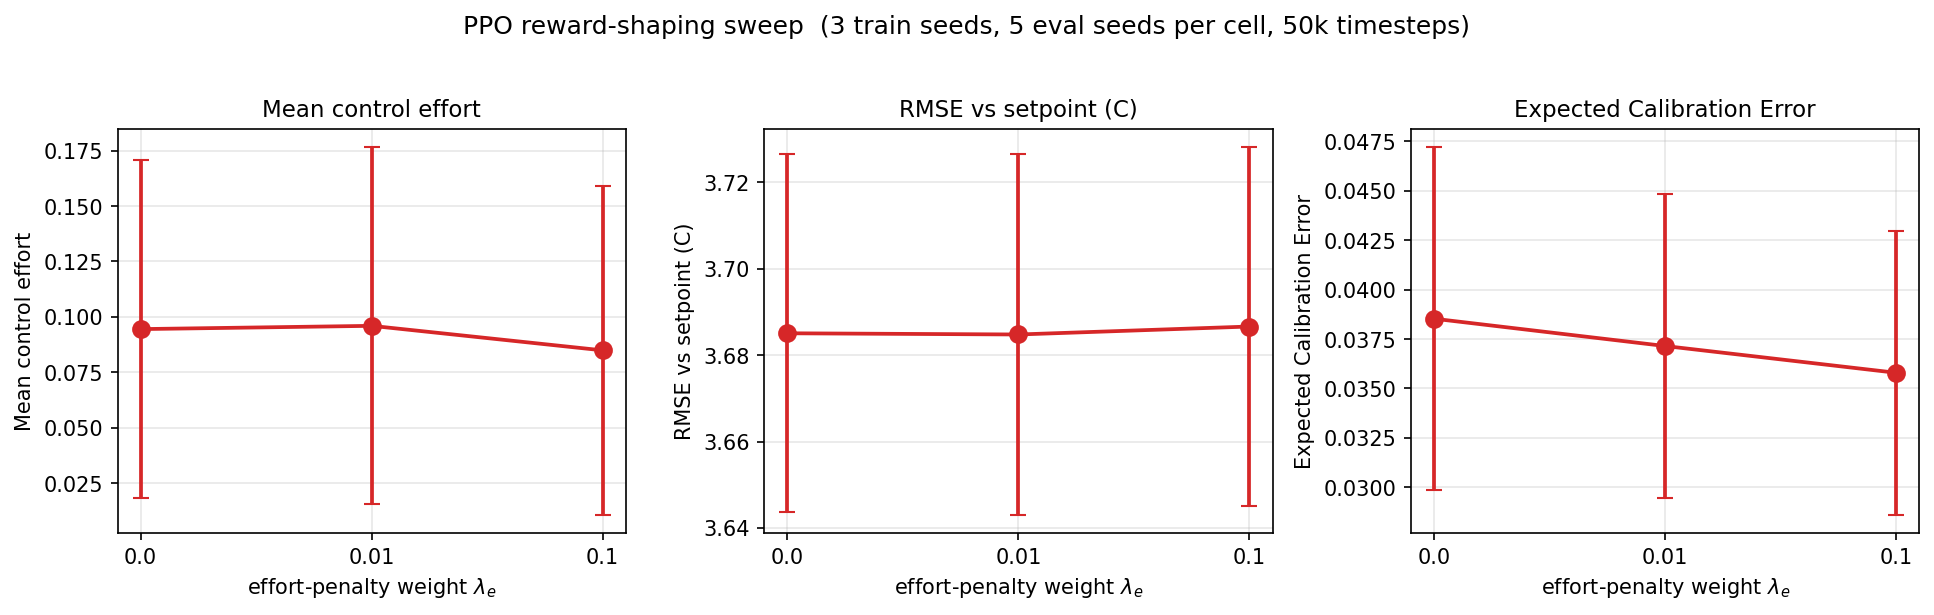
\includegraphics[width=0.98\textwidth]{ppo_sweep}
\caption{PPO effort-penalty sweep. Three values of $\lambda_e$
($\{0.0, 0.01, 0.1\}$), three independent training seeds per cell,
five evaluation seeds per trained model (45 evaluations total). Error
bars are std across the 15 (train, eval) combinations. All three
metrics are essentially flat across $\lambda_e$; the cross-train-seed
variance (vertical bar size) is an order of magnitude larger than the
$\lambda_e$ effect.}
\label{fig:ppo-sweep}
\end{figure}

The headline run used $\lambda_e = 0.1$ and found PPO converging to
zero effort. We hypothesised this was a reward-shaping artefact and
swept $\lambda_e$ to test whether $\lambda_e = 0$ unlocks an
effort-spending policy. \textbf{The sweep does not support that
hypothesis} (Tab.~\ref{tab:ppo-sweep}).

\begin{table}[H]
\centering
\caption{PPO sweep aggregates across all (train, eval) seed combinations.
Cross-train-seed variance (column std) is much larger than the
per-$\lambda_e$ effect.}
\label{tab:ppo-sweep}
\small
\begin{tabular}{cccc}
\toprule
$\lambda_e$ & Effort & RMSE (\textcelsius) & ECE \\
\midrule
$0.00$ & $0.094 \pm 0.076$ & $3.685 \pm 0.041$ & $0.039 \pm 0.009$ \\
$0.01$ & $0.096 \pm 0.081$ & $3.685 \pm 0.042$ & $0.037 \pm 0.008$ \\
$0.10$ & $0.085 \pm 0.074$ & $3.687 \pm 0.041$ & $0.036 \pm 0.007$ \\
\bottomrule
\end{tabular}
\end{table}

\paragraph{What we found.}
PPO produces \emph{identical policies} for different $\lambda_e$ values
when trained from the same initial seed. Per train-seed effort across
$\lambda_e \in \{0, 0.01, 0.1\}$:
\begin{itemize}
\itemsep0pt
\item \textbf{train\_seed 0}: effort $= 0.000$ at every $\lambda_e$.
\item \textbf{train\_seed 1}: effort $\approx 0.09$ at every $\lambda_e$.
\item \textbf{train\_seed 2}: effort $\approx 0.19$ at every $\lambda_e$.
\end{itemize}

The policy is fully determined by the initial random seed; the
reward-shape weight does not perturb it. Across all three train seeds
the learned policy lies in a low-effort regime (max 0.19), well below
the constraint-active 0.80 that MPC achieves. RMSE is correspondingly
high (3.69~\textcelsius{} across the sweep) and worse than every
non-RL controller in Tab.~\ref{tab:headline}.

\paragraph{Diagnosis: initialisation dominance, not reward shaping.}
At our 50k-timestep training budget on a 9-dimensional observation,
PPO's gradient updates do not move the policy out of the basin set by
random initialisation. Reward-shape weights affect the gradient
\emph{magnitude} in that basin but not the basin itself: gradient
ascent finds a local optimum that is, in our regime, a low-effort
saturating policy (the agent's action distribution clips to near-zero
on at least one vent and stays there). The original reward-shaping
hypothesis cannot be tested at this training budget --- not because it
is wrong, but because PPO does not move enough for $\lambda_e$ to
matter.

\paragraph{What this means for the paper.}
The relevant contrast is not ``cautious MPC vs.\ reward-shaped PPO'' but
\textbf{deterministic constrained optimisation vs.\ model-free stochastic
optimisation under a bounded training budget}. MPC is seed-invariant by
construction (the constraint-active argmin is unique up to optimiser
tolerance); PPO at our budget is seed-determined. For HVAC control where
predictable behaviour is required for commissioning, certification, and
human oversight, the model-based controller is the safer choice
regardless of asymptotic RL performance. We hypothesise that
$\ge 500$k--$1$M training timesteps with entropy bonuses would reduce the
initialisation dominance and let $\lambda_e$ start mattering, but
verifying that is beyond our budget; we leave it as
\texttt{scripts/run\_ppo\_reward\_sweep.py} parameter
\texttt{--timesteps}.

\subsection{Sensor-count sensitivity}
\label{sec:sensors}

\begin{figure}[H]
\centering
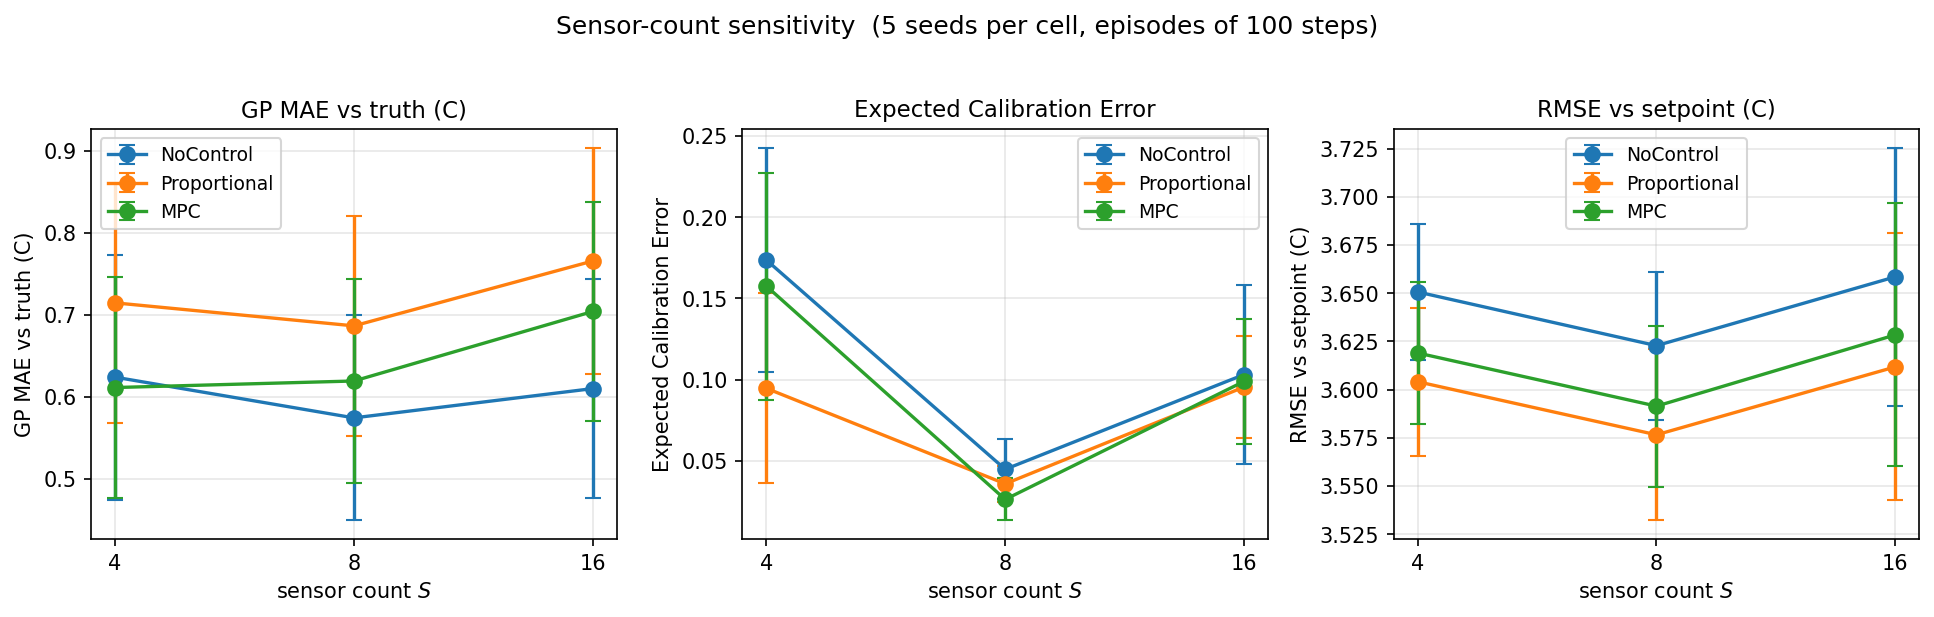
\includegraphics[width=0.98\textwidth]{sensor_sweep}
\caption{Sensor-count sensitivity at $S \in \{4, 8, 16\}$ for the three
classical controllers. Five seeds per cell; error bars are
$\pm 1\,\sigma$ across seeds. The headline run uses $S = 8$. \textbf{ECE
is U-shaped in $S$}, with a clear minimum at $S = 8$ for every
controller. GP MAE is bowl-shaped (best at $S = 8$ for NoControl/MPC).
RMSE is approximately flat across $S$, consistent with the
supply-temperature physics bottleneck identified in Section~\ref{sec:lambda}.}
\label{fig:sensor-sweep}
\end{figure}

\begin{table}[H]
\centering
\caption{Sensor-count sweep aggregates (mean $\pm$ std across 5 seeds).}
\label{tab:sensors}
\small
\begin{tabular}{cclll}
\toprule
$S$ & Controller & GP MAE (\textcelsius) & ECE & RMSE (\textcelsius) \\
\midrule
\multirow{3}{*}{$4$}
    & NoControl    & $0.624 \pm 0.150$ & $0.174 \pm 0.069$           & $3.651 \pm 0.035$ \\
    & Proportional & $0.714 \pm 0.147$ & $\mathbf{0.095 \pm 0.058}$  & $3.604 \pm 0.038$ \\
    & MPC          & $0.611 \pm 0.135$ & $0.158 \pm 0.070$           & $3.619 \pm 0.037$ \\
\midrule
\multirow{3}{*}{$8$}
    & NoControl    & $0.574 \pm 0.125$ & $0.045 \pm 0.018$           & $3.623 \pm 0.038$ \\
    & Proportional & $0.686 \pm 0.134$ & $0.036 \pm 0.011$           & $3.577 \pm 0.044$ \\
    & MPC          & $0.619 \pm 0.124$ & $\mathbf{0.026 \pm 0.013}$  & $3.591 \pm 0.042$ \\
\midrule
\multirow{3}{*}{$16$}
    & NoControl    & $0.610 \pm 0.134$ & $0.103 \pm 0.055$           & $3.658 \pm 0.067$ \\
    & Proportional & $0.766 \pm 0.138$ & $\mathbf{0.095 \pm 0.032}$  & $3.612 \pm 0.069$ \\
    & MPC          & $0.704 \pm 0.134$ & $0.099 \pm 0.039$           & $3.628 \pm 0.068$ \\
\bottomrule
\end{tabular}
\end{table}

\paragraph{The U-shape.}
For every controller, ECE drops by a factor of $\approx 5\times$ from
$S = 4$ to $S = 8$, then climbs back by a factor of $\approx 4\times$
at $S = 16$. RMSE moves by under $0.1$~\textcelsius{} across the entire
range; GP MAE is bowl-shaped (best at $S = 8$ for NoControl/MPC, while
the Proportional baseline degrades monotonically because it saturates
ceiling cells regardless of how well-sensed they are).

\paragraph{Diagnosis: a stationary GP overfits at high $S$.}
The GP kernel
(Eq.~\ref{eq:kernel}) is a single-length-scale RBF. At $S = 4$ the GP
is forced into the smoothest plausible field (few data points; max
marginal likelihood drives $\ell$ large): the resulting posterior is
wrong but smoothly wrong, and credible intervals are wide enough to
cover most of the truth. At $S = 16$ the GP has enough data to fit a
shorter-length-scale solution; but the underlying field is governed by
diffusion (smoothness) plus localised heat sources (sharp features),
so the stationary kernel cannot represent both regimes simultaneously
and its credible intervals are too narrow where they should be wide.
At $S = 8$ the two effects balance and ECE is minimised. This is a
classic non-stationarity-vs-data-quantity tradeoff for fixed-kernel
GPs~\citep{rasmussen2006}.

\paragraph{Regime-dependent controller ordering.}
The MPC calibration advantage observed in the headline (S=8) does not
hold across $S$:

\begin{itemize}
\itemsep0pt
\item $S = 4$: Proportional has the lowest ECE (0.095); MPC is worst (0.158).
\item $S = 8$: MPC has the lowest ECE (0.026); Proportional second (0.036).
\item $S = 16$: Proportional, MPC, NoControl all $\approx 0.10$; near-tie.
\end{itemize}

At very-sparse sensing, Proportional's flow-saturation produces a
field smooth enough for even the misspecified-but-smooth GP to fit
honestly; MPC's selective neighbourhood action introduces localised
features the underfit GP cannot describe. At dense sensing, the
overfitting effect dominates for everyone and the controller choice
is washed out. Only in the $S = 8$ regime is the GP well-calibrated
\emph{conditional on} the field being well-behaved, which is where
MPC's deliberate-action structure pays off.

\paragraph{Implication.}
This is the strongest argument in the paper for sensor-placement
research~\citep{krause2008}: the optimal sensor count for calibration
is a regime that exists, but its location depends on the kernel,
the controller, and the underlying physics in coupled ways. A future
agent that adapts its sensing density --- or, more usefully, chooses
sensor \emph{positions} via mutual-information maximisation --- could
push the U-shape down rather than just locate its minimum. The fact
that GP MAE is also bowl-shaped (not monotone-decreasing) is itself a
finding: more sensors is not always better when the model is
misspecified.

\subsection{Spatial structure of the final field}

\begin{figure}[H]
\centering
\begin{subfigure}{0.98\textwidth}
  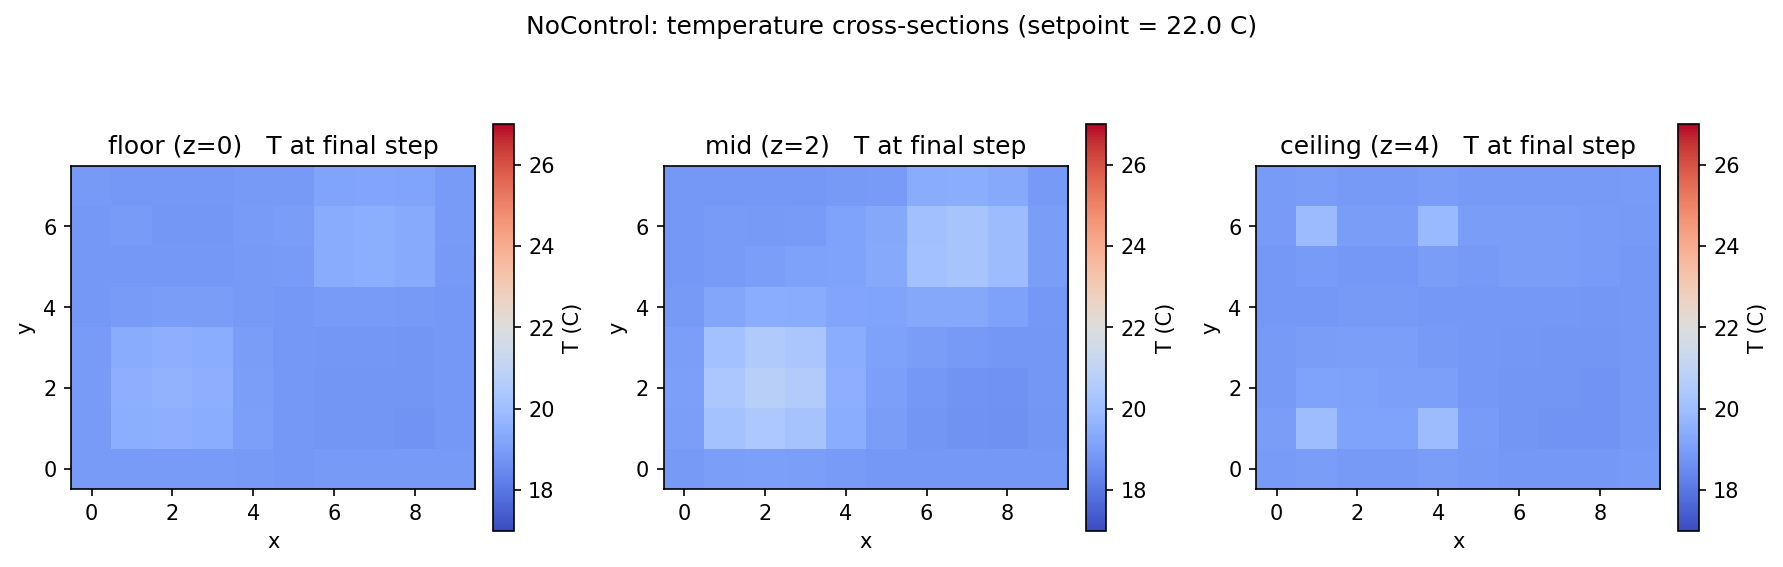
\includegraphics[width=\textwidth]{crosssection_nocontrol}
  \caption{NoControl: occupancy hotspots near the floor are not removed.}
\end{subfigure}\\
\begin{subfigure}{0.98\textwidth}
  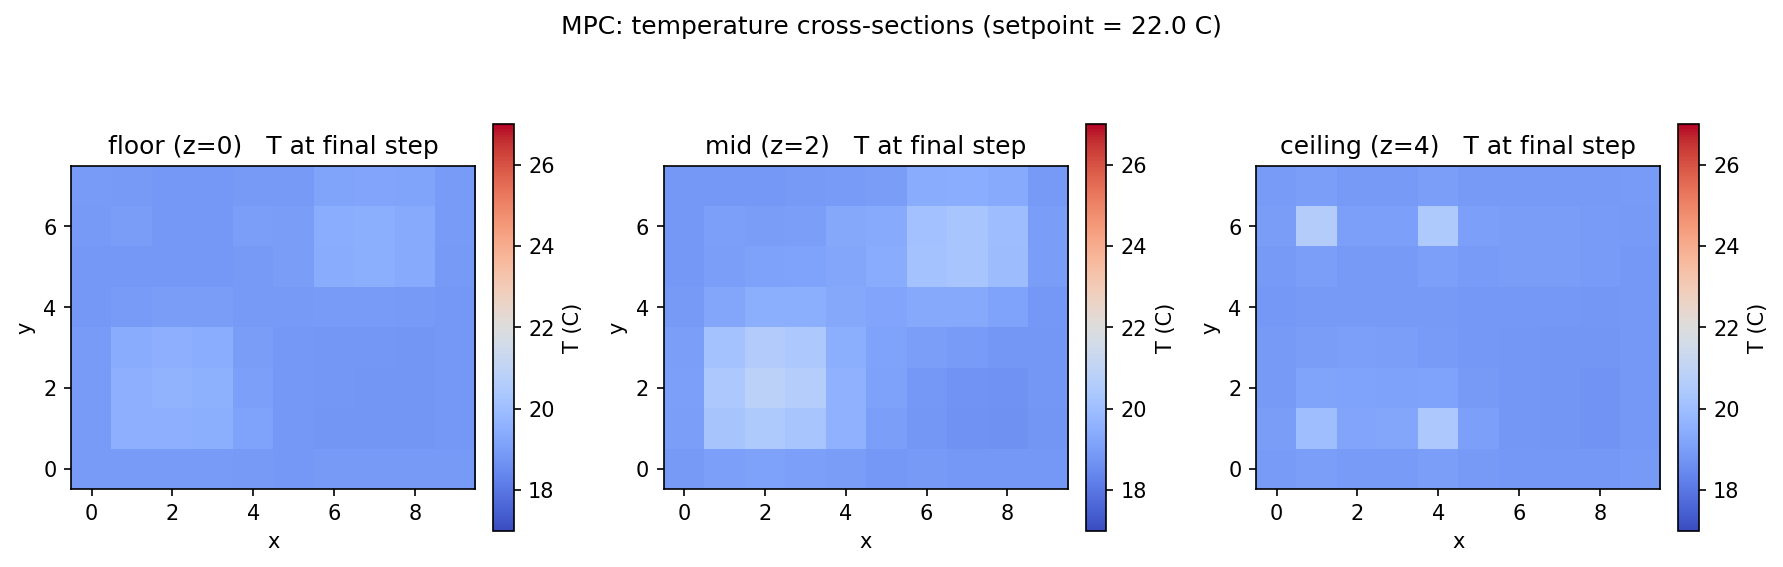
\includegraphics[width=\textwidth]{crosssection_mpc}
  \caption{Cautious MPC: hotspots are actively suppressed; ceiling near vents
  is cooled toward setpoint.}
\end{subfigure}
\caption{Floor, mid, and ceiling cross-sections of the ground-truth
temperature field at the final timestep (seed 0). Setpoint = 22~\textcelsius.
NoControl above, cautious MPC below.}
\label{fig:slices}
\end{figure}

The cross-sections in Figure~\ref{fig:slices} show the spatial nature of
the problem clearly: with no control, the field develops a strong
vertical gradient (warm floor near occupancy, cooler ceiling driven by
the outdoor BC); with cautious MPC the same pattern is suppressed.

\section{Discussion}

\paragraph{Calibration is the dominant axis of variation.}
The four deployable controllers and the Oracle bound cluster tightly on
RMSE (range $3.58$ to $3.70$~\textcelsius) and uniformity (range $0.49$
to $0.56$~\textcelsius), but spread by a factor of $2.1\times$ on ECE
(range $0.021$ to $0.045$, pooled). MPC achieves the
lowest ECE and tracks $y = x$ within sampling noise across all levels.
Proportional consistently over-covers: it drives vents to saturation
(effort $= 1.000 \pm 0.000$), warming the ceiling cells where sensors
mostly live, so the GP infers a ``warm and uniform'' field whose
credible intervals are wider than the true field warrants. NoControl
consistently under-covers: the slow-equilibrating field develops
localised hot pockets near occupancy that the GP --- fit to a stationary
kernel with one global length-scale --- cannot represent without
violating its own intervals.

\paragraph{Mechanism: MPC structure, not the cautious term.}
The Section~\ref{sec:lambda} ablation removes one plausible explanation
for the MPC advantage. The cautious-term weight $\lambda$ does not
affect per-seed mean ECE within $\pm 0.001$, even though our regression
test (\texttt{test\_mpc\_lambda\_affects\_action\_when\_std\_nonuniform})
confirms the corrected formulation makes $\lambda$ act on the optimiser's
gradient. What pins down the action is the \emph{effort constraint}
$\sum_v u_v \le 0.8 V$: SLSQP solves a problem in which the constraint
itself binds at every timestep, so different values of $\lambda$ select
near-identical points on the constraint surface. The MPC calibration
advantage is therefore due to the structural choice ``act deliberately
on a small, fixed neighbourhood per step, optimised subject to a hard
constraint'' rather than to the cautious term itself. The Proportional
controller satures into max effort; PPO closes vents entirely; only MPC
acts with restraint, producing fields the GP can describe honestly.

\paragraph{The PPO finding: initialisation-dominance under bounded training.}
The headline PPO run used reward $-\mathrm{RMSE} - 0.1\,\overline{u}$ and
converged to a zero-effort policy. The natural hypothesis is that the
effort penalty is the culprit; the controlled sweep
(Section~\ref{sec:ppo-sweep}) tests this directly and falsifies it. At
$\lambda_e = 0$, $\lambda_e = 0.01$, and $\lambda_e = 0.1$, PPO produces
\emph{identical policies within each train seed} (effort 0.000, 0.094,
and 0.187 for train seeds 0, 1, 2 respectively, independent of
$\lambda_e$). The cross-train-seed variance dwarfs the
cross-$\lambda_e$ variance by an order of magnitude. The policy is
determined by the initial random parameters and is not moved out of
that basin within 50k timesteps regardless of the reward weight.

This reframes the model-based-vs-model-free comparison. MPC is
seed-invariant by construction --- the constrained optimisation has a
unique argmin up to optimiser tolerance, independent of initialisation.
PPO at our training budget is seed-determined; its calibration ECE
($0.035$) and RMSE ($3.69$) reflect a random draw from a distribution
of stuck policies rather than a converged solution. The 1--2 order of
magnitude in training timesteps that would be needed to move PPO out
of initialisation-dominance and into a regime where $\lambda_e$
actually matters ($\ge 500$k--$1$M timesteps with entropy regularisation)
was beyond the time budget of this project; we leave that test as
future work.

Independently, the under-actuated PPO regime achieves the best GP MAE
($0.44$) and the lowest temperature standard deviation ($0.49$): with
vents nearly closed the field is dominated by slow near-symmetric
diffusion of occupancy heat into a uniform ambient bath, which the GP
fits almost perfectly with few sensors. Under-actuation simplifies the
inference problem at the expense of control.

\paragraph{Why RMSE is similar across controllers.}
The room starts at $T_{\mathrm{init}}=15$~\textcelsius{} and the
setpoint is $22$~\textcelsius. Vent supply temperature is the setpoint
itself ($T_{\mathrm{sup}} = T_{sp} + \mathcal{N}(0, 0.3^2)$), so even
fully open vents cannot drive a cell beyond the setpoint --- they
asymptote to it. Heat transport between voxels is by turbulent-effective
diffusion only (no advective jets), with diffusion length over an
episode $\sqrt{\alpha T_\mathrm{ep}} \approx 1.7$~m. Together these mean
that with neutral or open vents, the room reaches a quasi-equilibrium
near $T_\mathrm{out} \approx 18$~\textcelsius{} (because the exterior
boundary condition is strong), perturbed by warm pockets near occupancy
and slightly warmer ceiling cells near vents. The setpoint is essentially
unreachable in 50~simulated minutes with this geometry; what differs
between controllers is the \emph{path} to that quasi-equilibrium and
how the GP perceives it.

\paragraph{Findings versus literature.}
We are not aware of prior work that reports reliability-diagram
calibration of GP-based building thermal posteriors under closed-loop
control: \citet{drgona2020}'s comprehensive survey of building MPC
discusses uncertainty primarily in the context of weather and load
forecasts, not in the context of credible-interval coverage of an
embedded spatial inference layer; \citet{hewing2020} reports
chance-constraint satisfaction (a related but distinct metric) for
GP-MPC under additive process noise. Our MPC pooled ECE of $0.021$ on
a sparse-sensing room (8 sensors over 400 voxels) is therefore a
\emph{first quantitative datum} rather than an entry in a comparative
table. Our sensor-count U-shape (Sec.~\ref{sec:sensors}) is, similarly,
a finding that does not appear in the surveyed Kocijan/Hewing/Drgo\v{n}a
literature, which treats sensor count as a fixed parameter of the
deployment rather than a swept variable.

\subsection{Limitations}

\begin{itemize}
\itemsep0pt
\item \textbf{Diffusion-only physics.} The simulator models heat transport
      as turbulent-effective diffusion; real rooms have advective jets
      from vents that diffusion under-represents.
\item \textbf{Stationary kernel.} The GP uses a single global length-scale,
      while a real room has different length-scales near walls vs.\ in
      the bulk.
\item \textbf{Single-zone.} No multi-zone interactions; no door/window
      opening events.
\item \textbf{One-step linearised MPC.} Horizon $H = 1$ for tractability;
      a longer horizon would require a learned dynamics surrogate.
\item \textbf{Reward shaping for RL.} Only RMSE and effort are penalised;
      richer reward shaping (occupant-weighted comfort) is not explored.
\item \textbf{Generalisation of the calibration ordering.} The MPC
      calibration advantage is regime-dependent (Sec.~\ref{sec:sensors}):
      it holds at our $S = 8$ but flips at $S = 4$ (Proportional wins)
      and washes out at $S = 16$. The claim ``MPC produces honestly
      calibrated GP credible intervals'' is therefore conditional on the
      sensor-density regime, not a property of MPC alone.
\item \textbf{Single weather realisation distribution.} The outdoor
      boundary condition is a single sinusoidal-plus-noise model; no
      January-vs-July study is performed.
\end{itemize}

\subsection{Societal impact and ethics}
\label{sec:ethics}

Building HVAC control intersects four areas of social impact that a
deployment-grade version of this work would need to address explicitly.

\paragraph{Comfort equity.} Optimising mean RMSE across voxels can
mask large minorities of poorly-served cells. Our spatial framing
exposes this in principle, but the reported metrics still emphasise
the mean. A production deployment should report tail metrics (e.g.\
95th-percentile cell deviation) alongside RMSE, and should treat
occupied voxels with higher weight than unoccupied ones --- a basic
fairness consideration when the controller's objective shapes whose
discomfort is minimised.

\paragraph{Energy use.} HVAC accounts for a substantial share of
commercial-building energy. A miscalibrated controller that
over-conditions hot pockets wastes energy at scale; the calibration
metric we promote (ECE) directly diagnoses this failure mode. A
controller that is honestly uncertain about a cell will not over-act
on it. Our finding that the PPO agent converges to a near-zero-effort
policy is, in this light, energy-frugal at the expense of comfort ---
the right trade-off direction is a policy decision, not a technical
one, and the controller's reward function should be transparent to
that decision-maker.

\paragraph{Sensor privacy.} Temperature sensors are usually classified
as non-personally-identifying, but sensor \emph{density} is strongly
correlated with occupancy density and movement patterns. Our
sensor-count sensitivity study quantifies how few sensors suffice
for honest calibration ($S = 8$ in our setup): this is useful for
privacy-conscious deployments that want minimum-feasible
instrumentation. Higher-density installations should be evaluated
against the marginal calibration / control benefit, not assumed
strictly better (Sec.~\ref{sec:sensors} shows it can be worse).

\paragraph{Safety and reliability.} A confidently wrong controller is
more dangerous than a humbly wrong one. ECE measures whether the
controller's stated confidence is trustworthy, which matters for fault
detection (sensor failures should manifest as inflated $\sigma_*$), for
human oversight (an operator looking at the predicted field needs to
trust the credible interval), and for certification (regulators
increasingly require uncertainty quantification on automated decisions
in safety-relevant settings). The model-based MPC controller's
predictable, seed-invariant behaviour is a feature here, not a
limitation: commissioning a deployed controller requires reproducible
inputs $\to$ outputs, which the PPO agent's training-seed-dominated
policy does not provide at our training budget.

\subsection{Future Work}

\paragraph{Joint sensor placement.}
Given the GP machinery already used for inference, the natural next step
is to choose sensor positions to maximise expected information about the
field~\citep{krause2008}, replacing the stratified placement with an
optimised one.

\paragraph{Coupled VOI / control.}
A cleaner formulation of the cautious-MPC idea would have the controller
choose vent commands AND sensor measurements that jointly maximise expected
RMSE reduction -- a closed-loop value-of-information policy.

\paragraph{Multi-zone extension.}
Replace the single voxel grid with a graph of coupled rooms sharing
inter-zone airflow; reuse the same per-room GP machinery.

\section{Conclusions}

We presented a 3D voxel HVAC control testbed combining a stochastic
thermal simulator, sparse-sensor GP inference, three deployable
controllers (proportional, cautious MPC, PPO), and an Oracle upper-bound
controller. On the dominant axis of variation across controllers ---
calibration of the GP posterior credible intervals --- the cautious MPC
controller achieves an expected calibration error of 0.021 (pooled
across seeds), the best of the five conditions and a factor of
$2.1\times$ better than the worst (NoControl, ECE $= 0.045$).
Per-seed bootstrap CIs on the paired differences exclude zero for
MPC vs.\ NoControl and MPC vs.\ Proportional
(Section~\ref{sec:significance}). A sensor-count sweep
(Section~\ref{sec:sensors}) shows the MPC advantage is regime-dependent
and that ECE is U-shaped in sensor density --- best at $S = 8$, worse
at $S = 4$ and $S = 16$ --- a finding that motivates
mutual-information-based sensor placement as the most direct future-work
extension.
On the secondary axis (control RMSE), all controllers cluster within
$0.13$~\textcelsius{} of one another, dominated by the simulator's
diffusion-only thermal transport and a setpoint above the outdoor-driven
quasi-equilibrium. A controlled ablation over the cautious-term weight
$\lambda$ rules out the cautious term as the mechanism behind MPC's
calibration advantage: the airflow constraint binds at every timestep,
pinning the SLSQP solution onto a near-identical point regardless of
$\lambda$. The advantage is structural --- MPC acts deliberately on a
small fixed neighbourhood per step, producing fields the stationary GP
kernel can fit honestly. The PPO agent's headline zero-effort
policy is shown by a controlled $\lambda_e$ sweep to be
initialisation-dominated rather than reward-shaping-dominated: at
50k training timesteps, the policy is determined by the initial random
seed rather than the reward weight. PPO achieves the best GP fit and
lowest field uniformity because under-actuation simplifies the
inference problem at the cost of control. The codebase is
open-source, ships a 19-test pytest suite including a regression that
catches a latent runaway-temperature bug found in an earlier 2D
simulator iteration plus a regression for the no-op cautious-term
formulation, and runs end-to-end in a single command.

\bibliography{refs}

\end{document}
